% $Id$
%
%\chapter{Sample implementation -- Cactus}
%
% \mycitation{\txextsf{if purchasers [of word95] need to read [word97]
%   files they can buy an upgrade }.}{William H. Gates III}{\textsf{??}}


\chapter{\textit{Cactus} - a framework for web based document
  conversion and presentation}

\label{cha:cactus}
%\label{sec:cactus}

As mentioned in
\myvref{sec:making-it-as-easy-as-possible-for-authors-to-write-in-docbook}
it would be beneficial to have a simple, server based tool for
automatic conversion of a DocBook XML document into a set of formats
suitable for printing and web publishing, in order to relieve the
author of the chores of installing and maintaining the rich
environment necessary for a full set of commands for conversion of
the documents.

\textit{Cactus} is a such system for automatic conversion of
documents, images and other files into other formats.  Originally
prompted by the inability to view Microsoft Word files directly under
Solaris and Linux, but it turned out that the XML and SGML file
formats suffers from many of the same problems as Word in terms of
available viewers on non-Windows platforms, etc.  and that such a
generic framework for doing these conversions could be a very powerful
tool.

The Cactus system is my proof-of-concept implementation of such a
framework which can do document conversion and publication without any
intrinsic knowledge of the data in question, and in a way which is
basically transparent to the users by letting them use it as a simple
service where they use the tools they know.

% This chapter explain the Cactus architecture,
% \myvref{cha:cactus-sample-filter-sets} list a small set
% of external filters I have implemented to provide basic
% image and printjob transformations, after which I talk about the
% functionality of Cactus which has been considered but omitted in this
% initial proof-of-concept prototype.

The goals for Cactus were:

\begin{itemize}
\item Publishing documents must be as \textit{easy as
    possible} for authors.

\item The publishing process should be \textit{fully
    automatic}, without the need for human web masters.

\item The software base required from the audience should be
  \textit{as small as possible}.

\item The amount of intrinsic knowledge hard-wired into the
  system should be as small as possible.

\item In order to let Cactus use as many external programs as
  possible, the execution environment for these must be very
  flexible.

\item In order to have as many external programs available as
  possible, it is important to use an
  \myurl{http://www.opensource.org}{Open Source} platform.  
\end{itemize}

The above mentioned goals have been fulfilled to my
personal satisfaction even though the program turned out
differently than I originally envisioned. Cactus is today a
system which:

\begin{itemize}

\item Accepts electronic documents from many sources

\item Applies filters repeatedly to convert each document to
  as many other forms as possible

\item Allows easy access to the documents through a web
  browser

\item Provides a public service -- all information is
  available to everyone

% \item Allows documents to expire if they are not intended
%   for long term storage

\item Capable of using most utilities which can be executed from a
  command line, as filters.

\item Runs under the Redhat 6.1 Linux distribution.  
\end{itemize}

I have used Linux due to its wide availability, the fact that most
Open Source programs run under Linux, and my familiarity with the
system, but Cactus should run under any modern Unix variant with Perl
and MySQL.  For full functionality Java and Apache with the JServ,
mod_perl and mod_php extensions must be available.

Due to an underestimate of the effort needed to program the
database, I have not implemented as much of
the Cactus system as I would have liked to.

\section{Philosophy}
\label{sec:cactus-philosophy}

The Cactus philosophy is related to the
\myurl{http://www.acme.com/software/pbmplus/}{\texttt{pbmplus}
  software package from Jef Poskanzer} which is a very
powerful image manipulation package, based on three
\textit{very} simple image formats (namely PBM, PGM and PPM
for binary, gray-scale and color images respectively).  The
formats are understood by a lot of filters manipulating
these images (these may be piped together to combine
effects), and a number of conversion programs to and from a
large set of common graphics formats.  This approach has
proven to be very successful indeed, and Cactus functions as
the arbiter for applying such \textit{filters} to
\textit{items} in order to do the conversions and
derivations to make the files that the users require.

Cactus works with items which are considered to be data
streams with attributes owned by somebody.  Cactus itself is
only working with the data as a file containing raw data
with a MIME-type, and calls externally defined filters (may
be any kind of program that converts an input file to an
output file) to interpret and manipulate the information
inside as appropriate.

The database tables used by Cactus provide a number of
attributes which may be interpreted and set by the various
filters.  This allows the \textit{presenter} filters to
provide better and more informative views of the items.

By using an underlying database for data storage it is
possible to have several programs simultaneously do
gathering, conversion, derivation, compacting and
archiving of data while presenting data as web pages
responding to user needs. Experiments have shown that a
modern home PC is sufficient to run Cactus for a small work
group with a limited set of filters.

% By providing suitable \textit{examiners} of documents, which can
% extract classificational information it is a simple task to provide
% functionality similar to Yggdrasil.

% Cactus is as such not an application but a
% \textit{framework} for handling and converting documents
% without any intrinsic knowledge about the

% configuring a lot of filters which
% can transform documents from one form to another based on
% \textit{MIME-types} which is gaining momentum for a simple,
% standard way of specifying the content of a file.  MIME was
% first used by e-mail programs, and was later adapted in the
% HTTP-protocol underlying the world wide web.

\section{Why the name \textit{Cactus}?}

Please see~\myvref{fig:viggo-cactus} for a Danish explanation.

\myimage{gr/viggo-2}{The origin of the name
    Cactus.}{viggo-cactus}


\section{Cactus seen from the users perspective}
\label{sec:cactus-seen-from-the-users-perspective}

\myimage{gr/cactus-main}{The Cactus entry screen}{cactus-main}

% \myimage{gr/overview}{The basic idea behind
%   Cactus.}{overview}


\myimage{gr/cactus-ten-most-recent}{Ten most recent
  submissions}{cactus-ten-most-recent}

\myimage{gr/cactus-splitted-email-from-lars}{The status page of the
  ``Lidt Guf''-email from Lars Dalgaard.  The email contains a print
  layout in a scaled and a non-scaled PostScript
  file}{cactus-splitted-email-from-lars}

\myimage{gr/cactus-generated-pdf-from-lars}{The PDF-rendering of Lars'
  print layout (named ``Lidt Guf'')}{cactus-generated-pdf-from-lars}
  
For a user, Cactus is intended to be a black box, where documents are
inserted and the converted results are viewed in a browser.  As the
users use their usual tools to interface with Cactus, it is easy to
get the general idea about how Cactus works. A normal document
publication would be like this:


\begin{enumerate}
\item Submit the document to Cactus by one of many ways, like sending
  it as an attachment to an email or by printing it to a virtual
  printer.

\item Wait a few minutes.

\item Go to the Cactus home page and locate the upload.  There is a
  list of recent uploads pr user, and a quick list listing the very
  most recent uploads (see~\myvref{fig:cactus-ten-most-recent} on
  page~\pageref{fig:cactus-ten-most-recent}).
%   [An unimplemented
%   option is to email the user when the requested document conversions
%   have been completed]

\item The status page for the item shows all the files that Cactus
  have generated (see \myvref{fig:cactus-splitted-email-from-lars} on
  page~\pageref{fig:cactus-splitted-email-from-lars}).  The versions
  needed of each item can be viewed and downloaded.  URLs to items can
  be mailed to others for them to view, and other versions of items
  can be downloaded if so needed.
\end{enumerate}

\section{Design}
\label{sec:cactus-design}

\textit{The single most important design decision in the Cactus system
was to store all data -- including the commands to work with the
documents -- in a database!}

The impact on the way to do things, and my \textit{thinking} about how
to do things have been truly immense!

Previous projects used flat data files, and moving to using a modern
SQL database instead made the following benefits
possible:

\begin{description}
\item[Multi-programming] -- the database manages that several programs
  may access the data at the same time.
\item[Atomic updates] --  there is no chance that clients may access
  incomplete data by reading data another process is writing before it
  is done.  This makes the clients simple.
\item[Network accessibility] -- clients are not confined to run on the
  same computer as the database.
\item[Language independence] -- clients may be written in any language
  supported by the database.
\item[Easy retrieval of data] -- data handling is abstracted into
   simple ``SELECT'' and ``UPDATE'' statements, returning rows of data
   which are undisturbed by other processes.

\item[Easier programming] -- a lot of the tedious house holding is
handled by the data base.

\end{description}

As a direct result of these possibilities Cactus is now a system
evolving around database tables, and several programs working
simultaneously driven by the data in the tables.  I have identified
the following types of programs which should be running all the time
(and sleeping when they have nothing to do):

\begin{description}

\item[Validators] -- validates whether the content
  of the item is conforming to the MIME-type provided and
  the data valid.  If not, a MIME-type is synthesized
  according to filename and content.

%   If
%   not, or if a MIME-type is not provided, an guess is made to the
%   MIME-type based on the filename and file content, and this
%   synthesized MIME-type is then validated.  If that fails


% conforms with the is consistent with the MIME-type, and is it conforming to the
%   standard.  (Can a gzip-stream be decompressed? is a PostScript file
%   parsing correctly? etc.).  If a type is unknown, guess MIME-type
%   from filename and/or contents, and validate it.  If all fails,
%   assign a type of application/octet-stream.

\item[Extractor] -- looks \textit{inside} an item to look
  for references, embedded files and other kinds of data
  which can be extracted.  A reference may be a URL or an
  email address in a signature.  Embedded data could be a
  uuencoded image in a Usenet posting.

\item[Converters] -- create another version of a given item
  \textit{fast}.  These are intended for conversions of data
  with users waiting, like \texttt{pnm} to \texttt{png}.
  Compression schemes are normally rather time consuming and
  compression should generally be postponed for idle
  periods, where compressors are run.


%   These should generally be designed
%   to be as fast as possible, since these will be called from
%   CGI-programs with users waiting.  Avoid compression (gzip should
%   maximally be level 1).

\item[Derivers] -- create irreversibly
another item from one or more
  originals, like generate \texttt{dvi}-files
  from one or more \texttt{tex}-files.

% A deriver can ask for a conversion.
%For efficiency reasons, several computers could run derivers for
%Cactus.

%   This could be a multi-part MIME file which should be assembled into
%   a fresh original.  It could be a DVI file from several source files
%   (tex files and images).  These should generally be reasonably fast,
%   since their speed specifies how fast a new item can be made
%   available to the system.

\item[Compressors] -- Reduce the size of a converted item if
  possible, by employing any built-in compression schemes
  defined in the format of the item.  Sample formats are
  \texttt{png} which uses gzip-compression and \texttt{tiff}
  which uses LZW-compression.  A compressor may not change
  the MIME-type of an item.

%\item[\textsf{Optimizers}] --

% A converter is usually designed for being usable in
%   a real-time interactive setting (also called being fast), which
%   normally means that the result is sub-optimal.  An optimiser
%   complements this by doing a suitable optimisation step whenever the
%   system is sufficiently idle.  This could be running "pngcrunch" on
%   PNG files (which yields 30\% on Ghostscript output), or "tifftotiff"
%   on TIFF files.  The idea is that the file is still the same basic
%   type, and can be used without further modification.  It is an
%   "in-place optimisation".  Some file formats are using the gzip
%   compression scheme internally.  These would not benefit further from
%   archiving.

\item[Archivers] -- moves compressed items which has not
  been used for a long time into long-term storage, leaving
  only the meta-data.  This keeps the database files small.

%   This would typically be running "gzip -9" on the content, creating a
%   new entry (with a new mimetype), and marking the item as decachable.
%   The dearchiving process must be fast, since it might be needed by a
%   deriver without notice.


\end{description}

These are complemented by

\begin{description}
\item[Gatherers] -- gathers items from "outside" Cactus and
  enters it in the "incoming" table with an appropriate
  MIME-type and an owner.  Optionally an expiration date, a
  suggested filename and a comment can be provided. A
  data gatherer could accept email, emulate a printer, retrieve
  Usenet articles, etc.

\item[Janitors] - cleans up whenever the system is otherwise
  idle, or when the cache is full.  Converted items can be
  emptied of content, originals can be archived by being
  moved into off-line storage.  Expired items can be purged
  completely from the database, along with all their derived
  items.

\item[Presenters] - extracts data from the database, and
  presents them.  Possible presenters could be CGI-scripts,
  or  PHP3-documents.

%  The page should be cut in smaller pieces to
%  allow easier processing by Unix Netscape.
\end{description}

% \myimage{gr/xexample}{The processing of an email with a GIF
%   and a compressed tar-archive attached}{xexample}

\subsection{Example: Dissection of an email with two attachments}

\begin{figure}[htbp]
  \begin{center}
\begin{verbatim}
  0) "Hello, here is the
      files, I promised you"       -[*]-+-->  1) text/plain
     [pamela.gif]                       !        "Hello, here...."
     [myfile.tar.gz]                    !
                                        +-->  2) image/gif
                                        !        name:  pamela.gif
  * - use MIME::Tools to                !
      extract attachments               +-->  3) application/gzip
                                                 name:  myfile.tar.gz
                                                       !
      +------------ [ run gunzip, and decide ] --------+
      !               that this is a TAR-file
      V
  4) application/tar
     name: myfile.tar -------------[**]-+-->  5) text/plain
                                        !        "This is the real image,
                                        !         and a drawing by Anders"
  ** - unpack with tar, and decide      +-->  6) image/png
       the MIME-type for each           !        name: pamela.png
       file inside                      !
                                        +-->  7) application/octet-stream
                                                 name: mypcb.s01
\end{verbatim}
    \caption{The processing of an email with a GIF and a compressed tar-archive attached}
    \label{fig:xexample}
  \end{center}
\end{figure}


The processing of an email with a GIF image and a compressed
tar-archive containing a text file, a PNG image and a file in an
unknown file format, is shown in \myvref{fig:xexample}.  The
following steps happen when the email is processed by Cactus with the
proof-of-concept filters, and a functioning validator:

\begin{itemize}
\item The \texttt{message/rfc822} examiner is invoked and decides that
the MIME-message contain three parts: the text of the email, the
GIF-image and the compressed tar-archive.  This information is
forwarded to the \texttt{message/rfc822} extractor which extracts and
inserts these three items into the \texttt{items} table (along with
scheduling any possible derivations).

\item No entry in the \texttt{examiners} table exist for either the
\texttt{text/plain} or the \texttt{image/gif} MIME-types.  No further
processing.

\item The \texttt{application/gzip} MIME-type is a container with a
file inside.  The validator decides that this is a tar-file, with the
MIME-type \texttt{application/tar}.

\item This is again a container, which the \texttt{application/tar}
examiner decides to contain three files, which is validated to be a
\texttt{text/plain}, \texttt{image/gif} and -- since the validator
doesn't know it -- the default MIME-type for an unknown binary stream:
\texttt{application/octet-stream}.
\end{itemize}



In an ideal world we have infinite storage and infinite CPU-speed,
meaning that everything would be done instantly when we need it.
Since that is clearly not possible, it is necessary to find a fair
schedule for doing things, without overloading the system.  Cactus
uses a simple cost-based scheduler for derivations in the
\texttt{workqueue} table, based on expected CPU-time used for a given
derivation.  The ``cheapest'' derivations are then done first, leaving
very expensive ones for times when the system is otherwise idle.  This
pricing system would also be used to ask for immediate execution of
conversions which users request directly.

% \ttextsf{ What to do when the system runs so full that
%   archiving cannot be done fast enough.  Can data be moved
%   to "outside storage?".  }

None of this information is hardwired into Cactus.  All
filters are stored in appropriate tables, as listed with the
individual types.
%Full descriptions of each are present in
%the implementation section.

\subsection{Data gathering}

% NOTE:  Expanded graph to make it more readable!

%\myimage{gr/gather}{The data pathways into the
%  \texttt{incoming} table in Cactus. }{gather}

\begin{figure}[tbhp]
    \begin{center}
      
%       \ifx\pdfoutput\undefined
% % dvi
% %        [Graphic: \href{#1.png}{#1}]
%         \includegraphics[scale=0.4]{#1}
%       \else
% % pdf
%         \includegraphics[scale=0.4]{#1}
%       \fi
      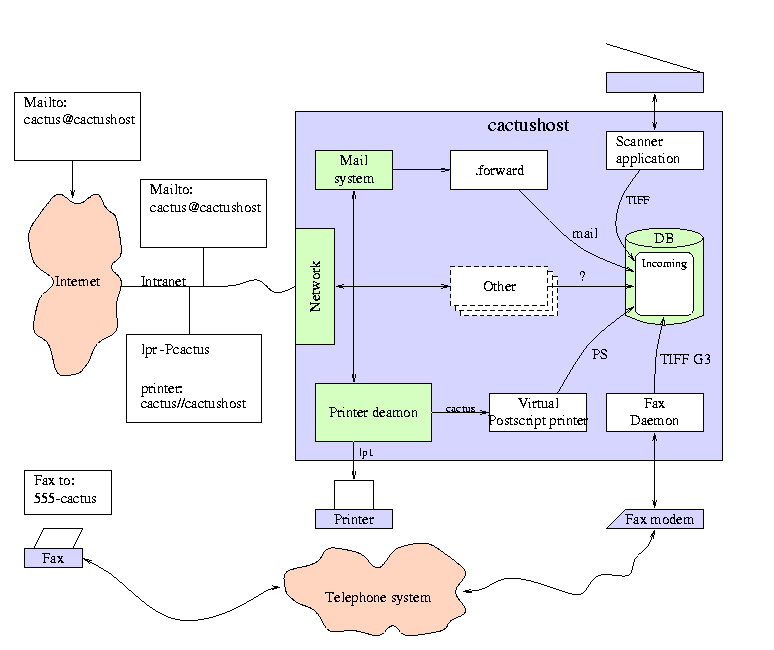
\includegraphics[scale=0.7]{gr/gather} 
%      \includegraphics{#1} 
      \caption{The data pathways into the \texttt{incoming} table in Cactus.}
      \label{fig:gather}
    \end{center}
  \end{figure}

Data can be gathered by just about any process that is able
to open a connection to the Cactus database.
\myvref{fig:gather} shows a combination of email, printing,
voice modem and scanning.  Some possibilities might be:


\begin{description}
\item[Email] -- a user may easily submit any file, by
  attaching it to an email which is sent to a virtual Cactus
  user.  For the proof-of-concept implementation this was
  \texttt{cactus@asserballe}
  (\texttt{cactus\%asserballe@mip.sdu.dk} for users outside
  of MIP).

\item[Virtual Printer] -- Cactus provides a virtual
  PostScript printer accessible from both Windows and Unix,
  which acceps printjobs that are inserted directly in the
  database instead of being printed out.

\item[Scanner] -- A scanner may produce one or more sets of
  images (one per page) which belong together.

\item[A drag-and-drop directory] -- A Windows \textit{file
    share} is provided in which users may put any file that
  is then moved in the database by a periodically checking
  daemon.  A similar directory is available to Unix users as
  an NFS-exported directory where users may create their own
  files, but not modify others.


\item[Fax] -- A fax-modem may be connected and used to
  gather faxes.  Information from the modem regarding phone
  number of the sender (as well as any other provided by the
  phone company) may be recorded along with the actual
  bitmap.  The bitmap may be printed directly, in order to
  emulate a regular fax.  If Optical Character
  Recognition-filters are installed, a text version may be
  generated which may be integrated in a full text search
  facility.

\item[Voice mail] -- The same fax-modem may be used as an answering
machine, and the recorded messages stored in Cactus as a WAV file.
These could with great benefit be converted to MP3 files and emailed
to people automatically or made available through the web.

\end{description}

Each of these must fill out as many fields in the
\texttt{incoming} table as possible (see
\myvref{tab:sql-incoming}) in order to provide as much
information as possible for later processing.

\textit{Note:} Only the email and printer data gatherers
have been fully implemented in the proof-of-concept
implementation.  The Scanner and Shared-directory gatherers
are on an experimental stage, and is not suitable for
production use.


\subsection{Examiners}

Cactus in itself have no notion of an item besides it being
a raw bit stream with a MIME-type.  With the addition of an
\textit{examiner} for a given MIME-type Cactus can be made
aware of whatever is inside an item.  An examiner must do
two things, and print the findings back on \texttt{stdout}
as lines of (MIME-type, space, value):

\begin{enumerate}
\item Provide information about the item in question and
  report it back to Cactus in order to have the attributes
  set in the database.  Each attribute should be listed as
  the MIME-type \texttt{x-cactus}/\textit{attribute}
  followed by a value, and printed to standard output.

\item Provide a full list of contained items within.  These
  should be printed with a value that uniquely allows the
  corresponding extractor to identify the item in question
  when given the MIME-type and the value.
\end{enumerate}

\myimage{gr/items}{How the examiner update an item, and provide
  information to the extractor (which erroneously is labeled as
  ``Deriver'' in the figure), which in turn extracts each contained
  item and insert it in the \texttt{items}-table.}{items}

Examiners are found in the \texttt{examiners} table (see
\myvref{tab:sql-examiners}).  ~\myvref{fig:items} show how an examiner
examines an item and return a list of the contents, Cactus updates the
item in question and forward a list of any contained objects to the
appropriate extractor which then in turn extracts the items the examiner
found, inserts them in the database flagged for later examination, and
schedules all the derivations possible in the
\texttt{workqueue}-table.

A sample examiner could be this which looks inside a PostScript file
to extract the title, if any:

\begin{verbatim}
perl -lne 'if (/^%%Title: (.*)/) {print "x-cactus/title $1"}' {@source-name}
\end{verbatim}

as the start of a PostScript file contains comments of the form:

\begin{verbatim}
%!PS-Adobe-2.0
%%Creator: dvips(k) 5.86 Copyright 1999 Radical Eye Software
%%Title: rapport.dvi
%%Pages: 170
%%PageOrder: Ascend
%%BoundingBox: 0 0 596 842
%%DocumentFonts: CharterBT-Bold CharterBT-Roman CharterBT-Italic
%%+ CharterBT-BoldItalic
%%EndComments
...
\end{verbatim}

The Examiner listed, looks for lines starting with
``\texttt{\%\%Title:}'' and uses the rest as the title of the document
printed in the PostScript file.  The result is printed to stdout as a
``\texttt{x-cactus/title Extracted-title}'' pair.  

\subsection{Derivers}

A deriver derives a new item (with another MIME-type) from
an existing item, based on an entry in the \texttt{derivers}
table.  A derivation is intended for irreversible actions, like
\texttt{tex} to \texttt{dvi}.

If the source file was derived from a container, all other files in
the container which had a filename will be present in the source
directory as well.  In this way, files can refer to other files in the
same container.  This is useful for multi-file submissions, like
{\LaTeX}-files which may be split up in several parts, or use external
images.  (Note:  The current implementation of the deriver launcher do
only provide the single source file).

This sample deriver creates a PostScript file from a DVI-file:

\begin{verbatim}
PRINTER= dvips -Z {@source-name} -o dummy.ps;mv *.ps {@dest-dir}
\end{verbatim}



\subsection{Converters}

Converters are intended for different representations of the same
data, usually images.

It is possible to contain the same graphical information in a PNG file
as in a PPM file so it is only necessary to store one of these in the
system.   The other one can easily be regenerated.  Cactus keeps track
of the amount of CPU time each file has used, and uses this to decide
which version should stay.   A PNG file is compressed as opposed to
the plain PPM format, which means that the PNG file has required more
CPU-resources to create than the PPM file.  The easiest file to
regenerate would therefore be the PPM file, so it can be removed from
storage.

In general converters are very similar to derivers, with the exception
that they should be used for \textit{reversible} actions like
PostScript to PDF and vice versa.   The attributes of the different
formats are identical, except for the MIME-type and those describing
the physical file.

Converters are currently implemented as derivers.

\subsection{Compressors}

A compressor knows how to \textit{improve} the internal representation
of a given MIME-type, without changing its external characteristica,
i.e. a TIFF-file is still a TIFF-file after the compression.

The same conditions apply to compressors as to derivers, where the
output file must contain an optimized version of the item.  If the
generated file is empty it is ignored.

A sample compressor command line for \texttt{image/png} would be:

\begin{verbatim}
pngcrush {@source-file} {@dest-dir}/dummy.png
\end{verbatim}

It is up to the compressor to decide whether the output is better, and
only leave the output file if it is.

Compressors are not implemented in the proof-of-concept
implementation.



%\subsection{Optimizers}


\subsection{Archivers}

An archiver is used to \textit{move data away} from the main database.
It is only necessary to archive original items, as derived items can
be regenerated by the same steps that was originally taken.  Archiving
does not mean that the item is removed from the current database -- it
is merely a process which stores copies of data elsewhere.  This
allows janitors to quickly discard items in the main database, in case
of problems.


\subsection{Janitors}

Janitors cleans up the system by removing expired items, and
reclaiming space used by archived items.  When a given item has been
archived, a janitor is free to remove the data of the item in order to
reclaim space and keep the size of the database down.

\subsection{Presenters}

Presenters usually extract data from the underlying database and
present them to the user in one form or another, and is allowed to do
simple updates of the stored data if this does not interfere with the
other operations done by Cactus.  For example may a presenter update a
counter for how many times this item has been viewed, or store the
current time as the time when this item was viewed latest.

The easiest way for a presenter to return information is to do this
as XML, which may then be rendered with a generic site style sheet in
order to produce set of similar pages.  

\section{Executing external commands}

The following steps are taken, whenever an external command is to be
run by Cactus.  The given command has currently the following
replacements done (the syntax is inspired by the SQLProcessor and XSQL
servlets as they use the same form):


\begin{description}

\item[\{@source-dir\}] -- the name of the directory in which the
source file resides.


\item[\{@source-id\}] -- the value returned from the examiner from
  this contained item.  For ZIP-files an index number would be likely.

\item[\{@dest-dir\}] -- the directory in which Cactus expects to find
  the output file(s).
\end{description}

The following is guaranteed:

\begin{itemize}

\item The \{@dest-dir\} will be writable -- the deriver should not
write files anywhere else.

\item There is no guarantee on the amount on free space in the file
system.

\item If a deriver uses for longer than 60 CPU seconds it will be
terminated and the output discarded.  I have been unable to create a
similar hard limit on the memory usage which has proven fatal several
times when handling large images or incorrect input data.  The hard
limits are stated in the configuration file.

\item A process may be terminated unexpectedly.
\end{itemize}

There is currently no means for a deriver to specify that a derivation
could succeed later even if it fail now.

These rules are not enforced but are merely guidelines.

\section{SQL tables}

As mentioned previously, the single-most best design decision was to
use a database for all storage needs of Cactus.  All database tables
are deleted, created anew from scratch and populated with the
\texttt{src/sql/reset-tables.sh} command
(\myvref{sec:src-sql-reset-tables.sh}), which -- by means of the used
utilities -- uses the definitions in \texttt{src/config.pl}
(\myvref{sec:src-config.pl}) to ensure that all programs uses the same
definitions.

The following tables are used:


\begin{description}

\item[Incoming] -- This table (see~\myvref{tab:sql-incoming}) is used
by all data gatherers to store their data in as plain strings.  A data
gatherers should only accept information from known and trusted
sources, and fill out the \texttt{owner} attribute and as many others
as it can.  Currently the MIME-type must be set to a valid value too,
as the validators are unimplemented.  The
\texttt{src/cactus/process-incoming.pl} script reads all entries in
this table which does not have the \texttt{processed\_p} flag set,
decides the userid and mimeid fields based on the \texttt{users} and
\texttt{mime} tables (creates an entry if none exists), calculates the
MD5-hash value of the data stream and sets empty default values for
the rest of the fields and insert it in the \texttt{items} table.

  The \texttt{entered}-field is set automatically when it is inserted
  in the table.

\input{../src/sql/incoming}

%\item[compressors]
%  \input{../src/sql/compressors}

\item[Derivers] -- This table (see~\myvref{tab:sql-derivers}) contains
  a filter which convert from one MIME-id to another MIME-id (like
  \texttt{image/jpeg} to \texttt{image/gif}).  The \texttt{stdout}
  flag is 't' if the command in \texttt{filter} prints the generated
  output to the stdout pipe instead of a file.  The
  \texttt{cost\_base} and \texttt{cost\_pr\_kb} are values to estimate
  the CPU-seconds to execute the command based on the size of the
  file.  These values must currently be estimated manually.

\input{../src/sql/derivers}

\item[Examiners] -- This table (see~\myvref{tab:sql-examiners}) is a
combination of two functionalities based on the mimetype, namely the
\texttt{examiner} field containing a command to look inside a file of
the given mimetype and list the contents and attributes.  The
\texttt{extractor} is called for each item contained inside, with the
provided value from the examiner accessible as '{@source-id}'

This is done by the \texttt{src/cactus/examiner\_d.pl} program which
also takes each newly generated item and inserts all available
derivation paths in the \texttt{workqueue}-table for execution.  The
examiner\_d.pl program examines the newest additions first, in order
to make the system provide the most recently added data as quickly as
possible.

\input{../src/sql/examiners}

\item[Items] -- This table contains an entry for each submitted item,
  as well as each derived and converted item.

The following fields do currently have a meaning:

\begin{description}
\item[owner] -- the id of the user who submitted the document.
\item[mimeid] -- the id of the mimetype for the item

\item[original\_mimeid] -- the originally provided mimeid.
  \texttt{mimeid} is what the system figured out with a validator.

\item[derived\_from] -- this is the document that this item was derived
  from.  For originals, this points to themselves.
\item[original\_id] -- this is the original item that all derived
  versions can be generated from.
\item[MD5] -- the md5 value for the item.  In most cases this value is
  uniquely identifying the item.
\item[processed\_p] -- has this item been examined (and its contents
extracted)?

\item[cpu\_used] -- the accumulated cpu-usage for a given item.  This
  is measured - not estimated.


\item[entered] -- datestamp for when the item was entered in Cactus.


\item[accessed]  -- how many times have this document been shown?
\item[last\_accessed] -- \ldots and when was that?
\item[item] -- the raw data of the item
\end{description}

The remaining fields are currently unused, but have all a meaning
which is currently unimplemented.


\input{../src/sql/items}

\item[MIME] -- This table contains the mimetypes known to the system.
  When an unknown MIME type is encountered it is created.  All MIME
  types should be entered in lowercase to facilitate compliancy with
  the MIME standard.

\input{../src/sql/mime}

\item[Users] -- This table contains all users known to the system.  If
  an unknown user comes in, she is created.  No external way of
  validating users is implemented yet.  For full names it would
  feasible to create entries from the global user list from the
  computer system which Cactus will be a part of.  The
  proof-of-concept implementation was populated with the users of the
  MIP unix network.

\input{../src/sql/users}

\item[Workqueue] -- This table
contains scheduled derivations.  Since some derivations are much, much
more time consuming than others, I have chosen to have an attribute
containing ``expected CPU-time usage'' calculated by the Cactus
component which calls the extractor.  This attribute is the
size of the file multiplied by the \texttt{cost\_pr\_kb} added to
\texttt{cost\_base}. This works pretty good

\input{../src/sql/workqueue}

\end{description}

The \texttt{src/cactus/process-incoming.pl} is the only daemon that
actually puts new things in the \texttt{items}-table.  It is invoked
every 5 minutes from a cronjob.

When new, unprocessed items are discovered in \texttt{items} by
\texttt{src/cactus/examiner\_d.pl} it examines the content and
extracts any contained items which is then inserted in \texttt{items}
too.  All possible derivations of these new items, are then calculated
from the \texttt{derivers} table, and the CPU-time to be used is
estimated, and each conversion job is inserted in the
\texttt{workqueue}-table.  The \texttt{workqueue\_d.pl} daemon is
responsible for taking all jobs in sequence with the least expensive
job first.  This allows quick jobs to be finished quickly, while still
servicing large jobs whenever it is their turn.  This scheme is not
elaborate enough to guarantee that a job will be run, but in almost
all cases the system will do less at night, and will then be able to
do the large conversions that there was insufficient resources for
when requested.  As several processes run at the same time, the
precise order of the items inserted will flunctuate, making id-numbers
an unreliable method of identifying an item.  Here MD5 numbers are
better since these are only dependent  on the byte stream inside the
file.  Unfortunately you are not guaranteed uniqueness, but for most
situations it will work well.

Occasionally a conversion started by either examiner_d or workqueue_d
causes the script to crash (this mostly happens when a very large
image conversion uses all the memory and causes other programs to
request memory, receive an error and crash).   To allow the system to
cope, a \texttt{src/cactus/wrap.sh} script was written.  This script
takes an argument, namely the daemon which should be restarted after a
few seconds, to quicky reestablish functionality.  It would be natural
to move the process-incoming.pl script to be executed by
\texttt{wrap.sh}, since this proved a more flexible mechanism than the
original occasional cronjob invocation.

\section{Implementing a search engine}

A simple search engine can very easily be implemented, by issuing a
query like

\begin{verbatim}
select * from items where title like '%search-term%'
\end{verbatim}

This uses the SQL-syntax ``\texttt{LIKE '\%search-term\%'}'', which
can be embedded in any of the supported languages.   MySQL also
supports GNU regular expressions, but I have not investigated those,
as they are not part of SQL-92.

% See
% \myvref{sec:cactus-implementation-search} for an example.

For a production version, it is important that the calling program
ensures that the search term does not contain any meta-characters that
may allow a malicious user to do harm to the system.

Note: An example of why it is necessary to be careful, is the search
term
\begin{verbatim}
a\%' ; drop table "items";
\end{verbatim}

which, when used in the select-statement above,
is turned into
\begin{verbatim}
select * from items where title like '%a%'; drop table "items"; %'
\end{verbatim}
which contains two valid SQL-statements before a syntax error will
occur.  The second of these commands removes the \texttt{items} table
from the system, and is generally not something you want users to do
at will.

% \section{Overall view}
% \label{sec:cactus-overall-view}

% \section{Data flow}
% \label{sec:cactus-data-flow}

% \subsection{Input sources}

% \subsection{Output formats}

% \section{Daemons and SQL tables}
% \label{sec:cactus-daemons-and-sql-tables}

%%%%%%%%%%%%%%%%%%%%%%%%%%%%%%%%%%%%%%%%%%%%%%%%%%%%%%%%%%%%%%%%%%%%%%%%%%%%%%%%

\chapter{Implementation}

\label{cha:cactus-implementation}




\mycitation{The devil is real.  He lives inside C programs.}{Phillip
Greenspun}{\cite{phillipandalexsguidetowebpublishing} page 202}

% \textsf{Install a text/html -> text/plain, and application/pdf ->
%   application/eps filter, each eps can then be filtered to text/plain
%   with text2ps.  Make a search engine in the text/plain things, and
%   one that looks in any file}
% substrings of the title.  The search box is present on the
% proof-of-implementation main page (see \myvref{tab:cactus-main}),

This section describes the proof-of-concept implementation of Cactus.
See \myvref{cha:source-code-listings} for source code listings.

Even though the email data gatherer was working in November 1999, it
took a very long time to get the data model right -- it took me very
long to sort out that a file can be many things depending on how you
look at it --  and getting all the
parts to function.  Although I cut down on expectations, I still had
the prototype functioning so late (middle of March 2000) that I didn't have
time to train users and have them use what I had created.
Additionally making the XSLT-based presenters work properly took a
\textit{very} long time, since this technology does not look like any
other programming language I have encountered.

\section{Hardware/software considerations}

The Cactus proof-of-concept implementation has been implemented on a
standard PC with a Pentium 133 MHz processor, 128 Mb RAM, a 10 Gb
harddisk, a 3c509 Etherlink III netcard and a Matrox Millenium II
video card.

The PC is running a standard Redhat 6.1 Linux distribution (notably
MySQL was installed), with the Linux Java 1.1.8 JDK from IBM and a
recompiled Apache (1.3.9) with the latest mod\_perl, mod\_php3 and
ApacheJServ for running presenters.  Perl 5.6.0 was automatically
installed as part of installing the latest versions of MIME::Tools
from CPAN.

The \texttt{lpd}-daemon was configured to let all computers in the
MIP-network to print to the Cactus printer by listing them in
\texttt{/etc/hosts.lpd}, and \texttt{sendmail} to accept mail to
Cactus.



\section{Data gathering}


\subsection{Email}

\begin{figure}[htbp]
  \begin{center}
    \listinginput{1}{procmailrc}
    \caption{\~{}cactus/.procmailrc}
    \label{fig:cactus-procmailrc}
  \end{center}
\end{figure}

The \filename{\~{}cactus/.procmailrc} (see
\myvref{fig:cactus-procmailrc}) determines what happens with incoming
email to the Cactus user\footnote{For this to be activated, the mail
  transfer agent (like PostFix, qmail and sendmail) must have procmail
  enabled.  If the current MTA doesn't have that, then upgrade to
  PostFix.}.
\myimage{gr/cactus-original-from-lars}{The
  original version of a submitted email}{cactus-original-from-lars}


The listed actions logging to \texttt{work/_logfile}, submit the email
as standard input to the program \texttt{src/cactus/enter-document.pl}
with the MIME-type \texttt{message/rfc822} (which is the same as used
by Netscape, and allows the Netscape user to view any forwarded Usenet
message directly with enclosed files -- see
\myvref{fig:cactus-original-from-lars}), and store a copy in
\texttt{work/incoming-mail}.  The script opens the database, and
inserts the email into the \texttt{incoming} table, with the given
MIME-type, user and submittal date.

\subsection{Printing to Cactus}

Printing to Cactus is implemented by providing an alternative
\textit{output filter} to the Linux Line Printer Daemon system, which
captures all the output, prints nothing out, and submits the printed
files to the database instead.

As the virtual printer is expecting PostScript files (with the
MIME-type \texttt{application/postscript}) the only difficult problem
is identifying the user correctly.  As the lpd-system provide the
login of the user submitting the request, and the hostname from where
the request originated, the \texttt{cactus_rewrite_email} function in
\texttt{src/config.pl} can establish a fully qualified email address,
and whether the printjob is acceptable.

A common configuration could be expected to be that all computers
within a given network are allowed to print to Cactus.  Therefore all
user names must belong to the official network domain name, and an
email address can easily be determined.  Note:  The filter has the
power to veto any submitted printjob.

An unsolved problem is that occasionally several identical printjobs
are issued within one to two seconds.  This occurred to me when I
submitted printjobs from a Solaris machine -- several reasons are
possible.  My current approach is to ignore any but one of multiple
print jobs which were submitted within 1--4 seconds.  This is done by
looking at the timestamp and the MD5-value of the byte stream sent to
the printer.


\subsection{Fax and Voice mail}

Brief experiments was made with the
\myurl{http://www.leo.org/pub/comp/os/unix/networking/mgetty}{\texttt{mgetty+sendfax}}
software available for Linux, which captures incoming fax'es as TIFF
G3 files and incoming messages as audio files.  The TIFF G3 files can
then be considered either as individual images, or collected by call.
The audio files can be converted with \texttt{sox} and
\texttt{bladeenc} to MP3 files which probably is the most efficient
for long term storage.  An easy application could be emailing the
resulting MP3 files to the ``owner'' of the telephone line in
question -- 8 kHz audio files in mono compress rather well with modern
MP3 encoders.  An estimate is that such sound clips can be compressed
to 0.5--1 Kb/s.

Due to the lack of free phone lines at MIP this data gatherer was not
intended to be part of the installation there.  A Cactus installation
was planned for \myurl{http://www.how.dk}{Peter Favrholt} privately,
where this data gatherer would have been implemented and tested.

\subsection{Scanning}

A HP 6350 with an automatic document feeder was purchased for this
thesis.  The idea was to use Cactus to provide a fast and easy scanner
facility for public usage, by allowing everyone to lay a stack of
paper in the automatic document feeder, press the Scan button, and let
Cactus consider the whole batch as a set of images from the same
container.

This is a very good scanner and it works well with USB under Windows
98, and is supported by SANE (the Linux scanner project) when using
the SCSI-interface well enough to be used reasonably well in Gimp but
SANE crashes once in a while.  The automatic document feeder were not
well enough supported to warrant usage, and due to time constraints I
reluctantly decided to use the accompanying software under NT at
Dorthe Anickas machine instead of starting to enhance the ADF support
in SANE, by using the ``Shared-Directory'' approach.


\subsection{Shared directories on a network}

This solution requires a daemon to watch a given directory to see when
new files arrive, and move them into the database.

\begin{itemize}
\item For Windows clients this directory is made publicly visible by
  setting up SAMBA correctly for a commonly writable shared directory.
  
\item For Unix this is made by creating a setuserid directory which is
  world writable and mountable for all trustworthy servers.
\end{itemize}

\section{Derivers and converters}

These are implemented as executing one or more external commands, and
are described as they are used in the sample filter sets in
\myvref{cha:cactus-sample-filter-sets}.

\section{Examiners}

I only wrote examiners for two basic types, namely an email message
(\texttt{message/rfc822}) and a PostScript file
(\texttt{application/postscript}) but this was also sufficient to set
many document titles and dismantle email messages.  


\section{Presenters}

Presenters can be written in any language with access to the
underlying database.  Those employed in producing the proof-of-concept
prototype are listed in \myvref{sec:presenters}.  At least three types
of presenters can be imagined:

\begin{itemize}
\item Presenting an individual item.  The URL
\texttt{http://asserballe/\~{}cactus/get.php?id=XX} extracts the item
with the given ID from the database along with its MIME-type, and
return it to the browser.  Additionally the URL
\texttt{http://asserballe/\~{}cactus/get.php?md5=XX} is recognized
which is persistent across database rebuilds.

\item Presenting a query from the database: Through JDBC to any Java
  program, like the SQL-processor in Cocoon which returns a complete
  XML-representation of query results, which can then be manipulated
  with XSLT operations.  This is used to generate all XML-based
  information in the proof-of-concept implementation.   SQL-queries
  can also be handled directly by PHP3, on a line-by-line basis for each line in the
  result of the SQL-query, and by the DBI::MySQL module in Perl, also on a
  line-by-line basis.

\item Manipulating external data.   The php3 script producing the
  graphic titles (like the ``Cactus'' title of
  \myvref{fig:cactus-ten-most-recent}) did so with a text string and a
  True Type font.
  
\end{itemize}


All but two sample presenters for Cactus were written as very basic
XML-documents with embedded SQL-requests and a set of XSL-style sheets
to render the result into the general style used.  It is v

As the XSLT-process
allow the author to work with the whole table instead of the usual
line-by-line approach, you may




A presenter may be written in any language
which has a driver to access the database, and which can be called
from the webserver.   Most drivers work on a row-by-row based model of
the result, in the traditional way of ODBC or JDBC.

The easiest way to 
Currently Cactus does not provide presenting data based on
MIME-type.  There are the following ways to extract
information and show it to the users through a webbrowser:


\section{Database}

I have used the standard MySQL installation with Redhat Linux 6.1, and
created a Cactus user with full access from localhost.

The latest JDBC driver from \myurl{http://www.mysql.org}{MySQL
  downloads} were necessary to fix a bug showing up when working
  against the latest version of MySQL.


\section{Web server}

The web server configuration was as follows:

\begin{description}

\item[Apache] -- version 1.3.11.  I had trouble building this with
  dynamic linking, so a static version was used instead.  This
  requires all needed modules to be compiled in.  The stock Redhat
  does not have the JServ component available.

\item[mod_perl] -- version 1.21.   Embeds a Perl interpreter in the
  webserver for faster CGI scripts written in Perl. 

\item[mod_php] -- PHP 3.0.15.  Provides the facility to execute PHP3
    scripts. 
  \item[Apache JServ] -- version 1.1.  Allow Apache to execute
    servlets (needed for Cocoon).
\end{description}
  
Follow the installation instructions carefully, since it is a bit
tricky!  The standard httpd.conf for Apache was modified to recognize
the .php and .php3 file types, to use the jserv.conf file, to use the
/perl/ directory to point to script files in /home/cactus/src/modperl.



Note: A problem not solved was that it is possible to specify an
incorrect URL to Apache, similar to
\texttt{http://localhost/perl/bigscript.pl/foo/} which causes Apache
to look for a number of files in this path which appears to be a
directory.  For some reasons the perl/bigscript.pl is executed for
each path lookup, meaning that if this bigscript.pl performs a big,
slow operation running twelwe of these can basically block the whole
machine until the many simultaneous operations have finished.

I believe this is a bug in Apache, unless I have missed a
configuration parameter.




% \section{Making it all work under Linux}

% Source code

% If I get the time I will make this a literate form. Perl
%modules with the literate programing extension?


% \section{The design of Cactus}
% \label{sec:the-design-of-cactus}

% I set the following goals for Cactus:

% Cactus were two projects

% Today there are very few working procedures which are
% potentially available to any computer user at a very low
% cost:

% \begin{itemize}
% \item Printing a document
% \item Email an attachment to another user
% \item Fax a document
% \item Scan an image
% \item Receive a voice mail
% \end{itemize}

% All of the above can easily be done with a computer as the
% recipient, allowing it to capture the data sent.  The format
% preserving the most information is email with an attached
% file, as the others use a visual or audible representation
% of the original data.




% \section{Overview}

% My idea with Cactus was from the start to create a web-based
% facility which would ease the process of publishing and
% sharing information via the Internet.

% [The short comings of Yggdrasil]

% I set the following goals for Cactus: * Publishing documents
% must be as easy as possible for authors * The publishing
% process should be fully automatic, without the need for
% human web masters * The software requirements of the
% audience should be as small as possible * The system must
% run under Linux

% These goals have been fullfilled to my personal satisfaction
% even though the program turned out differently than I
% originally envisioned. Cactus is today a system which *
% accepts electronic documents from many sources * applies
% filters repeatedly to convert each document to as many other
% forms as possible * allows easy access to the documents
% through a webbrowser * provides a public service - all
% information is available to everyone * allows documents to
% expire if they are not intended for long term storage


\chapter{Cactus - sample filter sets}
\label{cha:cactus-sample-filter-sets}

This chapter lists several sample filter sets which provide a glimpse
of the possible ways to use the Cactus system, even with the current
limitation of a single input and output file.

The filters described here are listed in
\texttt{src/sql/default_derivers.txt}, which is loaded when the
database is rebuilt.


\section{``Print to PDF'' functionality}
\label{sec:network-adobe-acrobat-pdf-printer}

\myimage{gr/cactus-20000507-1}{Cactus view of a web page printed directly from
  Netscape}{cactus-20000507-1}

\myimage{gr/cactus-20000507-2}{The PDF-version of the printed web page
  }{cactus-20000507-2}



The Adobe Acrobat Portable Document Format is well suited for sharing
electronic versions of printable documents, and the Adobe approach to
creating these documents is for the user to either create a PostScript
file manually and run through the Acrobat Distiller, or to install an
alternative printer driver which can generate PDF-files directly.
Alternatively \myurl{http://www.ghostscript.com}{the GhostScript
  system} can be used to create PDF-files from PostScript files, and
vice versa.

By configuring a computer to submit PostScript jobs to the virtual
printer provided by Cactus and using GhostScript in two simple filters,
a similar functionality is achieved.

\subsection*{application/postscript to application/pdf (to file)}
% By using the Cactus virtual printer, any user can very easily send a
% PostScript file to Cactus, and by providing a \textsf{conversion?}
% between PostScript and PDF-file Cactus can provide the same
% functionality as Adobe Distiller with GNU tools only.

\begin{verbatim}
    "ps2pdf {@source-name} {@dest-dir}/{@source-name}"
\end{verbatim}

If Adobe Distiller is available on the Cactus host, it can be used
with this filter (note that this prints to stdout):

\begin{verbatim}
    "distill < {@source-name} "
\end{verbatim}


\subsection*{application/pdf to application/postscript (to stdout)}
% By using the Cactus virtual printer, any user can very easily send a
% PostScript file to Cactus, and by providing a \textsf{conversion?}
% between PostScript and PDF-file Cactus can provide the same
% functionality as Adobe Distiller with GNU tools only.

\begin{verbatim}
    "/usr/local/Acrobat4/bin/acroread -toPostScript <{@source-name}"
\end{verbatim}

Using Acrobat Reader to generate the PostScript produces better
looking results, and smaller PostScript files than using
\texttt{pdf2ps}.  Additionally, Postscript jobs which make HP-printers
restart, usually print without error if converted to PDF and then
printed from the Acrobat Reader.  I have found that it is important to
have the very latest version of the Acrobat Reader installed at all
times to ensure full compatability with the PDF-files generated on
Windows, (as well as being able to read the files on
\myurl{http://www.adobe.com}{the Adobe web site}).

\subsection*{Comments}

\begin{itemize}
\item For Windows users it is important to use a \textit{simple}
  PostScript driver, like the one for the Apple LaserWriter.  Other,
  newer PostScript drivers may use printer specific commands to
  initialize the printer.  If desired, the
  \myurl{http://www.adobe.com/support/downloads/pdrvwin.htm}{Adobe
    PostScript printer drivers} may be downloaded and used for this
  purpose -- note however that embedding True Type fonts requires
  using at least GhostScript 6.0 on the Cactus host for proper
  rendering.

\item The filters also work on emails.  See
  \myvref{fig:cactus-splitted-email-from-lars} and
  \myvref{fig:cactus-generated-pdf-from-lars} for the PDF-conversion
  of an Encapsulated Postscript file.

\end{itemize}

Even though these are very simple filters, they allow the user to
create PDF-files from any of their programs just by printing to a
virtual printer using a PostScript driver.  I expect this to be a \textit{very}
common use of Cactus in a production environment.

\section{Image conversion to GIF, PNG and JPEG}
\label{sec:image-conversion}

\myimage{gr/cactus-20000507-3}{An email containing a scanned image in
  BMP format}{cactus-20000507-3}

The philosophy behind the pbmplus package (as mentioned in
\myvref{sec:cactus-philosophy}) complements Cactus very well.  With a
few basic filters it is possible to do a wide range of image
conversions.  Due to the number of filters I have quoted the
unmodified definitions in \texttt{src/sql/default_derivers.txt} below
(Two lines have been wrapped to fit the margins).

\begin{verbatim}
    # PNM-> PNG, GIF,JPEG
    #image/x-portable-anymap,image/png,t,"pnmtopng -compression 1 {@source-name}"
    image/x-portable-anymap,image/png,t,"pnmtopng  {@source-name}"
    image/x-portable-anymap,image/gif,t,
      "<{@source-name} ppmquant -fs -quiet 200|ppmtogif -quiet"
    image/x-portable-anymap,image/jpeg,t,
      "pnmdepth 255 {@source-name} |cjpeg -maxmemory 16m"
    #
    # TIFF -> PNM
    image/x-tiff,image/x-portable-anymap,t,"tifftopnm {@source-name} "
    image/tiff,image/x-portable-anymap,t,"tifftopnm {@source-name} "
    #
    # GIF -> PNM
    image/gif,image/x-portable-anymap,t,"giftopnm {@source-name} "
    #
    # JPEG -> PNM
    image/jpeg,image/x-portable-anymap,t,"djpeg {@source-name} "
    #
    # BMP -> PNM
    image/bmp,image/x-portable-anymap,t,"bmptoppm {@source-name} "
\end{verbatim}


\myvref{fig:cactus-20000507-3} shows the result of using the ``Scan to
e-mail'' facility in the software accompanying the HP ScanJet 6350C to
send an email to the Cactus system.  The enclosed BMP file -- which a
standard web browser cannot preview directly -- is converted to GIF,
JPEG and PNG.


\begin{itemize}
\item BMP is highly inefficient for scanned images -- the JPEG file is 20
  times smaller.

\item It is possible to use the general pbmplus philosophy to convert
  images.  All recognized image formats have a deriver to the
  \texttt{image/x-portable-anymap} format, and just the ones which can be
  shown by a browser have a deriver to that format.   This works well.
\item The Cactus loop detection mechanism ensures that just the
  necessary derivers are invoked.
\end{itemize}

This works well, but requires that an entry exist for each and every
format supported.  Cactus does not yet support wildcards in the
MIME-types which would be handy here, since the ImageMagick package
has a generic \texttt{convert} command which accepts a very large
amount of image formats and can convert them to PPM.

It would also be nice to have a preview facility of the image in a
thumb nail view, as well as a rescaling facility.  This was considered
but found to be too cumbersome as long as Cactus just works with the
main MIME-type, where an image can only have \textit{one}
representation in a given format.

\section{Generating HTML, RTF and PDF from DocBook XML}
\label{sec:xml-publishing}


% \begin{table}[tbp]
%   \begin{center}
%     \begin{tabular}{|l|l|l|p{12cm}|}

% \hline\hline
% Source & Destination & ? & Filter (single command line)\\
% \hline

% text/xml & text/html & t
% &\texttt{\smaller"CLASSPATH=/home/cactus/src/jars/xt.jar: /home/cactus/src/jars/sax.jar:/home/cactus/src/jars/xp.jar
% /usr/jdk118/bin/java com.jclark.xsl.sax.Driver \{@source-name\}
% /home/cactus/src/docbook/html/docbook.xsl"}\\

% text/xml & text/x-fo & t&\texttt{\smaller
% "CLASSPATH=/home/cactus/src/jars/xt.jar: /home/cactus/src/jars/sax.jar:/home/cactus/src/jars/xp.jar
% /usr/jdk118/bin/java com.jclark.xsl.sax.Driver \{@source-name\}
% /home/cactus/src/docbook/fo/docbook.xsl"} \\

% text/x-fo & application/pdf & f & \texttt{\smaller
% "TEXINPUTS=.:/home/cactus/src/passivetex/: pdflatex '\&/home/cactus/src/passivetex/pdffotex' \{@source-name\}$<$/dev/null; pdflatex '\&/home/cactus/src/passivetex/pdffotex' \{@source-name\}</dev/null; mv *.pdf \{@dest-dir\}"} \\

% text/xml & text/rtf & f & \texttt{\smaller
% "SGML_CATALOG_FILES=\$HOME/jade-1.2.1/dsssl/catalog: \$HOME/sgml/catalog:\$HOME/sgml/docbook/db31/docbook.cat jade -t rtf -d \$HOME/sgml/dsssl/docbook/print/docbook.dsl \$HOME/jade-1.2.1/pubtext/xml.dcl \{@source-name\}; mv *.rtf \{@dest-dir\}"}\\
% \hline

%     \end{tabular}
%     \caption{Filters for DocBook publishing}
%     \label{tab:docbook-filters}
%   \end{center}
% \end{table}

Cactus can be used as a complete XML-typesetting and publishing engine
by creating suitable filters for each step in the process.  With a few
filters it is possible to have a DocBook-based system, which works
reasonably fast.  The sample DocBook document listed in
\myvref{sec:amanda-readme.xml} can be processed in the normal fashion
creating the tree of derived items shown in
\myvref{fig:cactus-20000506-3}, where each filter has been applied accordingly.

\myimage{gr/cactus-20000506-3}{The sample DocBook document listed in
  \myvref{sec:amanda-readme.xml} with derived
  versions}{cactus-20000506-3}

The filters must be on a single line, but have been wrapped and resized for legibility
\subsection*{text/xml to text/html (sent to stdout)}
{\footnotesize
\begin{verbatim}
CLASSPATH=/home/cactus/src/jars/xt.jar:/home/cactus/src/jars/sax.jar:/home/cactus/src/jars/xp.jar
/usr/jdk118/bin/java com.jclark.xsl.sax.Driver {@source-name} /home/cactus/src/docbook/html/docbook.xsl"
\end{verbatim}
}
This filter uses \myurl{http://www.jclark.com/xml/xt.html}{XT} to
apply the HTML-version of the
\myurl{http://www.nwalsh.com/docbook/xsl/index.html}{XSL DocBook Style
Sheets} and print the resulting HTML file to standard out.  See
\myvref{fig:cactus-20000506-4} for the result --  Note that a table of
  contents is generated and inserted at the beginning of the document.

\myimage{gr/cactus-20000506-4}{The HTML version.}{cactus-20000506-4}


\subsection*{text/xml to text/x-fo (sent to stdout)}
  {\footnotesize
\begin{verbatim}
CLASSPATH=/home/cactus/src/jars/xt.jar:/home/cactus/src/jars/sax.jar:/home/cactus/src/jars/xp.jar
/usr/jdk118/bin/java com.jclark.xsl.sax.Driver {@source-name} /home/cactus/src/docbook/fo/docbook.xsl
\end{verbatim}
  }

Again a rendering with XT, but this time to XSL-FO.  The FO target is
not as good as the HTML target, most likely because of limited
resources for development, and since this is a much less visible
target than the web oriented XHTML/HTML-4.0 targets.

\subsection*{text/x-fo to application/pdf (sent to file)}
  {\footnotesize
\begin{verbatim}
TEXINPUTS=.:/home/cactus/src/passivetex/:
pdflatex '&/home/cactus/src/passivetex/pdffotex' {@source-name}</dev/null
; pdflatex '&/home/cactus/src/passivetex/pdffotex' {@source-name}</dev/null
; mv *.pdf {@dest-dir}
\end{verbatim}
}

Currently the best results for rendering FO for printing is
\myurl{http://users.ox.ac.uk/~rahtz/passivetex/}{Sebastian Rahtz'
  PassiveTeX} with the
\myurl{ftp://ftp.cstug.cz/pub/tex/local/cstug/thanh/pdftex}{PDF-\TeX}
variant of {\TeX} to produce PDF files directly.  It must be called
twice to get cross references right.  Setting \texttt{TEXINPUTS}
informs {\TeX} where to find the files needed by the
\texttt{pdffotex}-format.

\myimage{gr/cactus-20000506-5}{The PDF version.}{cactus-20000506-5}

See \myvref{fig:cactus-20000506-5} -- The red print is
  the default for unimplemented tags in the DocBook XSL style sheet.

\subsection*{text/xml to text/rtf (sent to stdout)}
  {\footnotesize
\begin{verbatim}
SGML_CATALOG_FILES=/home/cactus/jade-1.2.1/dsssl/catalog:$HOME/sgml/catalog:$HOME/sgml/docbook/db31/docbook.cat
jade -t rtf -d $HOME/sgml/dsssl/docbook/print/docbook.dsl $HOME/jade-1.2.1/pubtext/xml.dcl {@source-name}
; mv *.rtf {@dest-dir}
\end{verbatim}
}

The RTF version is created by applying the DSSSL DocBook style sheets
to the XML file (which is why the \tag{!DOCSTYLE}-tag is present).
This filter requires a full DocBook SGML environment to be configured
in order to be usable -- the \texttt{SGML_CATALOG_FILES} informs Jade
where the various catalog files describing the setup are located.
Jade requires nothing but the \texttt{xml.dcl} file to be capable of
parsing XML-files.  The easiest way of getting a full SGML environment
is to install the files from the CD accompanying the DocBook guide
\cite{walsh-muellner:docbook-the-definitive-guide}.

\myimage{gr/cactus-20000506-6}{The RTF version.}{cactus-20000506-6}


See \myvref{fig:cactus-20000506-6} for the rendered output -- This is loaded in
  StarOffice 5.1 under Solaris, and has worked flawlessly in the word
  processors I have tried, including Word 97.






















\chapter{Cactus - what may the future bring?}

I have had a lot of ideas myself and received a lot of excellent
suggestions while developing Cactus.  Many of these were excellent,
but was postponed due to time constraints.  This overview should bring
an idea about what I envisioned when I started.

\subsection*{Generate data on demand}

Currently Cactus generates all possible derivations of each item by
applying all possible derivers when a given item is extracted, unless
such a MIME-type already has been derived from the original.

This generates a lot of formats that are never needed, so Cactus
should allow on-the-fly derivation of a given item to a given
MIME-type, while the browser waits.  If the derivation will take too
long (estimated from the cost variables stored with each deriver) the
user is notified and the derivation scheduled for background
execution.  When the item is ready, the user is sent an email with the
URL to the item.

Cactus should always try to generate \texttt{text/html},
\texttt{text/xml} and \texttt{image/png} versions of every item since
these are considered the standard formats which the user usually
selects.

When user preferences are implemented, the users should be able to
specify what standard derivations they expect and generate those
instead.

\subsection*{Use a seperate MIME-type for internal use, and have
  filter \textit{patterns}}

The basic idea of using the MIME-type of a document to identify what
Cactus is to do with the document, has proven sound, but is too
restrictive to do all the things I wanted it to

\begin{description}
\item[\textbf{Multi-resolution images}] -- It is frequently relevant
  to have images in several resolutions, like a high resolution image,
  and a thumbnail image in a set resolution.  Cactus can currently not
  distinguish between these different versions if they have the same
  MIME-type.  By providing a more elaborate MIME-type for internal use
  (like \texttt{image/png-300dpi} or
  \texttt{text/xml-docbook-3.15}) it is possible to provide more
  information and have a more refined set of filters.  As the example
  shows, this technique can also be used to embed the XML-dialect in
  the MIME-type allowing to have several different filters based on
  the XML-dialect used.

\item[\textbf{Patterns}] -- the \texttt{convert} program from the
ImageMagick program is capable of converting many, many image formats
to PPM.  In order to use \texttt{convert} as a generic image
conversion for unrecognized MIME-types, Cactus should be extended to
allow for MIME-patterns, like \texttt{image/*}.  This should be
extendable to allow the filters to use this information, like to use
the encoded size of an image.

\end{description}


\subsection*{Multi-file and container support}

Proper support of containers must be implemented.  The current state
of a single file without any of the other files in the original
container is not satisfactory, since it does not allow for the more
complex uses of Cactus, where multi-file documents are submitted
either as several attachments to the same email or as a ZIP-file.

For this to work, the validation mechanism must be fully implemented
first.

\subsection*{Email notification}

Users should receive an email notification when documents they
submitted themselves are ready.  The email should contain the precise
URL to the page describing all derivations of the item.

Multiple submissions should be collected together to avoid too many
small email in the mailbox, with a user definable time limit like 5
minutes or half an hour.


\subsection*{External documents}

Cactus should be able to deal with external documents directly.  The
meta-information is stored in the database, but the item is only
physically present elsewhere.

\subsection*{Active document surveillance}

Cactus should be able to put surveillance to an external document,
allowing the content in the database to be updated automatically to
reflect the new status.  The original submitter of the item may
optionally be notified of the new status.

This includes URL's extracted from documents, and Usenet references.
Possible uses could be that Cactus watched a discussion thread on a
news server, allowing the user to only look by when a new posting
enters a given thread.   Cactus should also be able to present a
threaded view of the whole discussion, similarly to the Usenet
interface at Deja.

\subsection*{Better Usenet support}

Cactus should be able to detect URL's and decode images found in
Usenet posting(like uudecode), and use these as any other derived
item.

% The most complete approach to URL decoding was posted by
% Abigail (a well known person in the Perl community) late 1999, and
% was a regular

\subsection*{Voice mail integration}

Cactus should be interfaced to a standard voice-mail capable modem,
allowing Cactus to create MP3 versions of messages which may be stored
in Cactus, and the URL to it emailed (in the usual fashion) to the
recipient.


\subsection*{Microsoft Word filters}

The \texttt{wv} program should be fully ported to produce 100\% valid
DocBook XML with SVG graphics (or TEI if the state of the FO style
sheets for DocBook does not improve).  This is largely independent of
Cactus as such, but will be an extremely important application.


\subsection*{A more generic search engine}

A search engine can be implemented in several ways -- I made a quick
implemention of a simple SQL-based search based on the title of the
document.  Another approach could be to blindly let a standard search
engine index all the possible pages, but that would definitively be
overkill and incrementing the counters without reason.

A reasonable compromise between indexing every thing and only indexing
on what we know to be meta-data, would be:

\begin{itemize}
\item Create a lot of filters to \texttt{text/plain}.  For example
  could
  \myurl{http://research.compaq.com/SRC/virtualpaper/pstotext.html}{pstotext}
  be used to extract the text for each page in a PostScript file.

\item
  Index the text pages, and let the search results point back to the
  original file from which the text was generated.
\end{itemize}

It would then be possible to locate a word in a PostScript file by
finding it in the text version, and then link back to the originating
page.  The \texttt{pstotext} authors claim it to be one of the best
tools for doing this, since it takes great care in converting the
letters-with-attributes back to ISO-Latin characters.  (The authors
wrote this utility for their
\myurl{http://research.compaq.com/SRC/virtualpaper/home.html}{Virtual
Paper} project -- it is worth a look)


\subsection*{Impose stronger restrictions on the filters}

There is very few restrictions on a filter, and I had severe problems
with rogue filters (which behaved according to specifications but
required too many system resources).  For example would a PPM to GIF
conversion normally be a question of calling \texttt{ppmquant} to
limit the number of colors used in the image to a number less than 256
(as GIF is palette based), and then calling \texttt{ppmtogif}.

For large numbers \texttt{ppmquant} ended up allocating so much memory
that it caused other processes to be denied the memory \textit{they}
needed for their execution, instead of just being limited to e.g. 16
Mb of virtual memory.  Processes like sendmail, apache and X, 
exit in such a situation which eventually leaves the system in a
useless state.  The problem was reproducible, meaning that every time
the database was rebuilt the machine slowly froze and eventually hanged.

The initial solution -- just to get going -- was to add more swap
space, and start looking for a way to set a hard limit with respect to
memory and CPU-usage.  The \texttt{ulimit} should be capable of
setting both, but I only managed setting the CPU-limit.  The machine
still runs with too much swap, and the system is noticeably slower than
it was initially.    I have not found the exact reason yet. 



% \chapter{Cactus - possible candidates for filters}
% \label{cha:cactus-possible-candidates-for-filters}









% % \subsection{Yggdrasil - a simple navigational framework}
% % \label{sec:yggdrasil}


% % The Yggdrasil system was designed to provide a simple, consistent
% % navigational framework around a dynamic set of web pages provided by
% % users, as well as providing a "recently changed pages"-list plus an
% % overview of pages written by each person.  This was a very successful
% % idea in the start, but gradually lost momentum due to these factors:

% % The development platform was changed from Unix to NT, which made it
% % much more difficult for the users to access their web-directories, as
% % these were no more a part of their home directory\footnote{The Apache
% %   webserver uses the ~/public\_html directory for the users personal
% %   web pages.  The transition to NT meant that the users - in addition
% %   to their normal file manipulations - should telnet to a Unix server,
% %   and change the file attributes every time the file was updated.  }

% % The internal document format became Microsoft Word, which at that time
% % could not be converted to HTML.  Such documents were therefore unable
% % to be published.

% % The users could trigger an update by sending an empty email to the
% % system, as well as rely on an automatic nightly update.  The trigger
% % mechanism was not brought along when the email system was converted to
% % NT.

% % New users was not informed about the system.














% ypx is from comp.sources.misc volume 40
% http://ftp.lth.se/archive/usenet/comp.sources.misc/volume40/ypx/

% compiles on solaris with "-lsocket -lnls".  does not compile
% on linux



% \section{Background}

% A major computer problem not solved satisfactory yet, is the
% ability for users to share information in spite of them
% using different hardware and software.  Even though the
% modern use of the Internet allow any two users to exchange
% files as attachments to email without any furter ado, it has
% not helped much in actually \textit{interpreting} the
% contents of these files.

% If a given user needs to use a given document, she needs
% software specific to the document format to interpret it.
% If another user needs the document, she needs software too.

% The most prominent word processor document format today is
% the Microsoft Word format, which is so complicated that even
% Microsoft has trouble with it (hence the quotation of this
% chapter).  Basically you need Word to use this format -- all
% other solutions provide inferiour results.  If you only need
% to read and print documents Microsoft provides a Word Viewer
% program for this, which require Microsoft Windows.

% Unfortunately, this is no help for those users who does not
% have Word, notably Linux users.

% \textsf{presentation and internet thingie}




% The Cactus system is an Open Source document conversion and
% presentation framework, which allows users to submit
% documents to a central server, which then uses a set of
% stored conversion filters to process the documents into
% other forms, notably HTML and other Internet formats.

% The version of Cactus described herein, have the following
% features:

% \begin{itemize}
% \item Convert documents to HTML versions viewable in a
%   browser
% \item Windows and Unix clients can use Cactus as a virtual
%   PostScript printer with automatic PDF conversion, and may
%   download the result directly or view the HTML-conversion
%   (making this accessible to platforms without Acrobat
%   Reader).

% \item Images can be resized and converted to a number of
%   formats like JPEG, TIFF, and PNG.
% \item Extensible and configurabele.  New filters can be
%   installed to convert from one MIME-type to another.
% \end{itemize}


% This runs on a single Linux machine, but any number of Unix
% machines may requests jobs to do if more CPU-power is
% needed.  \textsf{The necessary filters and a simple Java
%   client must be installed on each.  Will the support be
%   active?}.





% \textsf{ingen dokumentstandard.  ingen wp-producenter der
%   underst'tter det, ingen interessei at goere noget ved det,
%   ingen ting.

%   nu wp9 understoetter sgmlredigering, StarOffice er frit
%   tilgaengeligt paa mange platforme, osv osv}



% % \section{abstract}

% % \begin{quotation}
% %   The Cactus system fills a gap in the current integration of the web
% %   with normal office procedures, as it provides easy web publishing
% %   for occasional authors, by letting them submit documents in several
% %   ways with their usual software.

% %   The system automatically produces other versions of the documents on
% %   demand of the users reading the documents, as well as provide the
% %   navigational framework, relieving the local webmaster from these
% %   tedious and error prone tasks.
% % \end{quotation}

% \subsection{System description}
% squid: http://www.squid-cache.org/

% \framepage{15cm}{ Cactus is a sample implementation of the
%   following issues:

% \begin{itemize}
% \item \textbf{easy publishing} - users can publish via
%   email/fax/print/watch usenet/www which is processed into
%   the SQL database, and confirmed.

% \item \textbf{automatic conversion} - system will
%   automatically convert a given document to what the user
%   can see (or want).  Browser sends a capability string with
%   each request -- use that to provide stuff directly, or
%   generate a ``this is available'' summary.

% \item \textbf{automated navigational framework} - each
%   document has an annotation which tells Cactus where to
%   place it in the navigational hierachy.  The corresponding
%   navigational pages are automatically generated and updated
%   when new documents arrive.  This also ensures system
%   integrity without ``broken links''.
% \end{itemize}

% Implementation languages - possibly Java or Perl.  Perl
% chosen due to better library support (with source).  Rex
% thingie in Java.  How can MIME, TAR, etc be done in Perl
% (remember jubilations!).  Using Apache with Cocoon (perhaps)
% and MySQL.  Graph algoritms
% in~\cite{sedgewick-algorithms-in-c}.

% Good summary from 19991114.  Speed of PNG gzipping?  PNG
% uncompressed intiially and then later compressed by
% pngcrunch.  }

% http://photo.net/wtr/word.html Utilities: mswordview,
% xls2xml

% \subsection{Background}

% \framepage{15cm}{ Explain the history.  Yggdrasil to address
%   the need of an automatic webmaster $\rightarrow$ analysis
%   (seperate file written earlier).  Cactus to address the
%   difficulties of publishing information to Yggdrasil.}


% Explain Cactus as a successor to Yggdrasil.

% \subsection{Installation}
% Perlmodules.  MySQL server. SAMBA.


% [Rephrase following paragraph]

% I have concluded the following goals for CACTUS, in order to
% avoid repeating history:

% \begin{enumerate}
% \item "Ease of publishing" is crucial.

% \item Document preparations and transformations must be
%   fully automatic.

% \item The organisation using the system must be fully doing
%   so.

% \end{enumerate}

% \subsubsection{"Ease of publishing" is crucial}

% CACTUS uses two approaches in order to make publishing as
% easy as possible for the users, namely

% \begin{center}
%   Documents are accepted in their native format, and in
%   numerous ways.
% \end{center}

% Discussions with potential users showed [...] to be
% realistic ways in which CACTUS would be used:

% As a document storage for various versions of a document,
% being developed and emailed back and forth between authors
% and peers.  By allowing CACTUS to accept documents as email
% attachments, it would be very easy to enter each draft in
% CACTUS by including it on the list of authors or peers.  In
% this way the archival of the document in CACTUS is
% completely transparent.  As a fax machine.  When replacing a
% fax machine with a computer, it is very easy to send a copy
% of the temporary image of the fax to CACTUS, before printing
% it.  The fax system is then enhanced with the possibilities
% of the web, relieving the need for the physical copy.  As a
% printer.  Cactus provides a "printer", which makes a
% web-version out of any document the users can print.  Users
% can then share final versions of documents without requiring
% the recipients to have the software in question.  Either the
% Adobe Acrobat Reader can be used, or the primitive multiple
% image viewer in Cactus.

% The full list of the publishing methods in Cactus is listed
% [....]

% The users were primarily expecting to use these file
% formats:

% \begin{itemize}

% \item Word DOC and RTF files.  These are the storage formats
%   of the Microsoft word processor Word.
% \item HTML files.  The common format for the web.
% \item LaTeX files.  This typesetting program is very popular
%   with mathematically oriented academics.
% \item GIF, JPEG, TIFF and PNG images.  These and many more
%   are in common use.  Cactus use PNG internally [except
%   possibly for JPEG].  The full list of supported formats is
%   listed in the implementation section [see somewhere].
% \item PostScript and PDF files.
% \item Fax images.
% \end{itemize}

% \subsubsection{Document preparation and conversion must be fully automatic}

% There was a strong consensus amongst the users, that it
% would be very nice not to have to convert the documents
% manually every time they were to publish a document.
% Therefore Cactus accepts several document formats as
% described above, and abandons the requirement that the users
% should convert their documents to HTML before publishing.

% The system have some very different views on the documents
% depending on which representation the user needs - not all
% make sense for all documents:

% \begin{enumerate}
% \item The unaltered original.  This file is always
%   available, allowing users with the correct software to
%   continue working with it.

% \item A normalised version of a document.  This could be a
%   PNG version of a TIFF image or BMP image which can be
%   viewed by all modern browsers, and an XML version of a
%   document.  If a suitable encoding can be found, even
%   images and sound can be represented in XML so that this
%   does not overlap the textual representation.

% \item A visual representation of the original.  This is the
%   "look of the file", i.e. as it would look when printed to
%   paper, and allows users without the corresponding software
%   to view and print the contents.

% \item A textual representation of the original.  This is the
%   "meaning of the file", which could say that the line "foo
%   bar" is a level 2 heading, providing search capability.


% \item An audio representation of a "document".  This is e.g.
%   an message left on an answering machine.
% \end{enumerate}

% Conversions between all these document representation must
% be automated as much as possible.  [write about the Cactus
% framework for providing existing and future filter types].
% The normalised document is the only one created when a
% document enters Cactus - the rest are created on demand to
% avoid overfilling the underlying database, but cached for a
% reasonable time to improve performance.

% [....]


% The organisation using the system must be doing fully so.[
% rephrase]

% In order for such a system to be successfully used within an
% organisation, it is vital that the organisation is using it
% whole-heartedly.  [and more of the same].


% Note on derivers:

% A deriver is a pipeline which derives another version of an
% item.  E.g. PNG to GIF,

% \subsection{The implementation of Cactus.}



% Goals:

% \begin{itemize}
% \item Stable, well-known and remotely administrative
%   platform- Linux/Solaris
% \item Platform independence - the resulting system must not
%   be tied to Unix

% \item Modular - in order to minimise actual development,
%   software libraries should be used as much as possible.

% \item Extensible - it should be easy for the system
%   administrator to enhance functionality.
% \end{itemize}

% Choosing an implementation language:
% \label{sec:cactus-choice-of-language}

% Since platform independence was important for the system, it
% was quickly found that reasonable choices would include
% scripting languages plus Java.  Scripting languages are
% fully interpreted allowing a script to run on numerous
% platforms without change.  Java is the only compiled
% language with this property, due to the "Write once, Run
% everywhere" philosophy from Sun, plus the tight integration
% with Internet technologies in Java.

% Initially I wanted to write the core of Cactus in Java, and
% spent a couple of weeks evaluating the language but found
% that


% The mentality of the Java-community on the Internet, is very
% influenced by the shareware philosophy typical for the
% PC-user.  Everything useful cost money, source code is not
% revealed, and the general tendency is for large, stand-alone
% applications.

% Nobody had written a publicly available, stand-alone
% MIME-parser in Java.  Several RFC's should be implemented
% and tested, in order to get email-parsing in Cactus.

% The general level of abstraction is - in my opinion - too
% low in Java, while the "core language" is enormous.



% [?]



% Information extraction from items.



% A given document contains one or more items, which again may
% contain further information.  Cactus uses the MIME-type of a
% given item, to select the information scanning method with a
% fall back to the generic application/octet-stream examiner.

% The application/octet-stream is parsed for:

% The text is scanned for URL?s, either with the Tom
% Christensen urlify or the program posted or commented by
% Abigail.  These include ftp, http, gopher, mailto and news
% references.  These are stored as external references.

% The text/plain is parsed for

% uuencoded data in a text stream.  These start with ?begin
% \#\#\# name?, contain lines matching \#\#\#\#, and ends with
% ?end?.  Such a file is then assigned a validated MIME-type
% based on the name of the file, and entered in the system as
% a derived item.

% An text/html item is parsed for:

% normal references in \tag{a}-anchors.  While doing this, the
% text to be rendered is extraced and parsed as a text/plain
% stream, in order to get the sequence right (may be changed).
% The \tag{meta} tags are examined in order to extract
% keywords for the label.



% \subsection{Converters}
% \label{sec:converters}


% \subsubsection{Microsoft Word}

% The Microsoft Word DOC-format is widely used, but apparently
% so hard to use that even Microsoft have trouble doing it
% correctly, and the reason why Cactus was started in the
% first place.  I have spent a great deal of time looking for
% suitable software which could have been used with Cactus on
% the server side, and then testing it out.  \textsf{WINE}

% \begin{description}
% \item[Microsoft Word] -- The best solution would be able to
%   actually run Word itself, but apparently this is
%   integrated so well with Windows that it cannot run on
%   other systems like \myurl{http://www.winehq.org}{WINE}.
%   Since Microsoft previously have deliberately made the
%   Windows 3.1 version of Internet Explorer 4 unable to run
%   in the WinOS/2 subsystem for OS/2, I strongly suspect that
%   this is also the case here.

% \item[Viewer for Microsoft Word] -- the Word Viewer is
%   available for all Microsoft operating systems.  The 16 bit
%   version is reported by Usenet posters to behave reasonable
%   in WINE, and would be a good candidate for producing
%   PostScript printouts of Word documents.  It would require
%   a full Windows application to automate this, since it does
%   not support command line arguments.

% \item[Corel WordPerfect 8 for Linux] - This is generally a
%   very nice word processor, but the import filter for Word
%   crashed WP when I tried it with a large document.  Filters
%   should be better in WordPerfect 9, which is due for Linux
%   medio 2000.

% \item[StarOffice 5.1] -- the German office suite for several
%   platforms have excellent filters for importing Office
%   files in general, but cannot be automated from the command
%   line.  A StarBasic program must be written and invoked to
%   do the job -- a request on the StarOffice newsgroups for a
%   tool to do this, did not get any response.  Due to lack of
%   time I did not pursue this further.

%   Since I did the testing, Sun have bought StarOffice - most
%   likely since they need an network based office suite for
%   Java, which StarOffice provide with thin clients and a
%   Solaris based server - and promise to make the source
%   generally available.  This has not happened yet, but it is
%   currently the most likely alternative to the Microsoft
%   Office solution.

%   The StarOffice package is such a popular package that Sun
%   has a download counter on their main home page (which said
%   1,962,277 downloads as of 2000-04-03).


% \item[AbiWord] -- An Open Source word processor which is
%   part of the Gnome Office suite.  It was not able to parse
%   my test documents in Word.

% \item[wv] (previously mswordview) -- an Open Source Word to
%   HTML converter which currently do text well, but have
%   trouble with graphs which are converted to the WMF format.

% \item[Do-It-Yourself] - If you ask Microsoft very nicely,
%   you can get a copy of the Microsoft Office Binary File
%   Format Specification, and write a personal parser of Word.
%   It took Microsoft 6 months to answer my email request, and
%   then they just sent me the license twice with no
%   specification.  Second time they got it right.
%   Unfortunately, the license was so restrictive that I
%   decided not even to \textit{look} at the specification.

% \item[Majix] - This small RTF to XML converter written in
%   Java, can also parse DOC files when running in the
%   Microsoft Java Machine by invoking Word to save the DOC
%   file as RTF.  (Unfortunately it had serious problems with
%   RTF files generated by other programs).  It was easy to
%   customize it to generate DocBook XML.

%   If Majix could be called from Cactus with a DOC-file and
%   return the corresponding XML file a major goal had been
%   accomplished.  A test scenario was therefore made with a
%   remote telnet session to a NT-machine, where Majix was
%   invoked from the command line.  The test failed as Word
%   hung in the start up phase -- my personal guess is that
%   Word needs access to the GUI.  An installation on a MIP
%   server was not possible due to MIP system policy.

%   Additionally the company has not released a new version in
%   a year, and the license explicitely prohibits disassembly.

% \end{description}

% My intermediate solution has been to adapt the mswordview to
% output DocBook XML instead of HTML, which provides a
% text-only display.


% \subsubsection{{\TeX} and {\LaTeX}}

% \textsf{tex4h}


% \subsection{MySQL}
% On asserballe

% \begin{verbatim}


% create table incoming (when datetime, mime varchar(80), user
%   varchar(80), how varchar(80), filename varchar(255), comment varchar(80),
%   item longblob);

% +----------+--------------+------+-----+---------+-------+
% | Field    | Type         | Null | Key | Default | Extra |
% +----------+--------------+------+-----+---------+-------+
% | when     | datetime     | YES  |     | NULL    |       |
% | mime     | varchar(80)  | YES  |     | NULL    |       |
% | user     | varchar(80)  | YES  |     | NULL    |       |
% | how      | varchar(80)  | YES  |     | NULL    |       |
% | filename | varchar(255) | YES  |     | NULL    |       |
% | comment  | varchar(80)  | YES  |     | NULL    |       |
% | item     | longblob     | YES  |     | NULL    |       |
% +----------+--------------+------+-----+---------+-------+
% 7 rows in set (0.01 sec)


% \end{verbatim}

% \begin{itemize}
% \item \textbf{ wmf-anything}: libwmf (no fonts),


%   \myurl{http://ourworld.compuserve.com/homepages/kkuhl/}{KVEC}
%   (could not render the wmf files from wv),



%   \myurl{http://www.companionsoftware.com/PR/WMRC/WindowsMetafileFaq.html}{WMF
%     docs}

% \end{itemize}


% \section{Programs}


% \subsection{Linux - an operating system}
% \label{sec:linux}

% Linux was chosen as the development platform for these
% reasons:

% \begin{itemize}
% \item High degree of familiarity with the operating system
% \item Almost all Open Source software run ``out-of-the-box''
%   on Linux
% \item High performance Java Development Kit available from
%   IBM
% \item Remotely maintainable via X/telnet/ssh.
% \item Freely available from the Internet.
% \item Root access possible without interfering with MIP
%   security rules
% \end{itemize}

% These rules were also most likely fullfilled by any of
% FreeBSD/NetBSD/OpenBSD/Solaris x86, but I had already burned
% Redhat 6.1 on a CD for my portable, so there was no need to
% look any further.  Linux has been a very satisfactory
% choice.

% \subsection{Apache - a high performance web server}
% \label{sec:apache}

% There have probably been written more webservers than
% editors in the world of today.  My requirements were simple:

% \begin{itemize}
% \item Run Perl programs efficiently
% \item Run Java servlets efficiently
% \item Have a large user base in order to ensure program
%   availability
% \end{itemize}

% This basically left a single web-server, namely
% \myurl{http://www.apache.org}{Apache}, which is capable of
% running Perl CGI scripts very efficient with
% \myurl{http://perl.apache.org/}{the \texttt{mod\_perl}
%   module} (which uses a resident Perl interpreter combined
% with caching of the bytecode of previously encountered
% programs).

% If requirements were less, other webservers might have been
% applicable.  The
% \myurl{http://www.mortbay.com/software/Jetty.html}{Jetty}
% (Java Webserver capable of running servlets),
% \myurl{http://www.acme.com/java/software/Acme.Serve.Serve.html}{Acme.Server}
% and \myurl{http://www.roxen.com}{Roxen} (standard webserver
% with excellent graphics capabilities) webservers are just a
% few candidates for tasks with a less diverse need for
% scripting languages.  Servlet support is getting very common
% place.


% \subsection{Squid - a high performance web cache}
% \label{sec:squid}

% \myurl{http://www.squid-cache.org/Doc/FAQ/FAQ-20.html\#what-is-httpd-accelerator}{The
%   http-accellerator mode}


% \subsection{Cocoon}
% \label{sec:cocoon}



% \section{Filters}
% \label{sec:cactus-filters}


% \subsection{ps to pdf}
% \label{sec:filter-ps-to-pdf}

% \begin{description}
% \item[\myurl{http://www.adobe.com/products/acrdis/main.html}{Adobe
%     Distiller}] -- The reference PostScript to PDF
%   converter.

% \item[\myurl{http://www.ghostscript.com/}{Ghostscript}] --
%   This is a PostScript interpreter which has gained wide
%   usage.
% \end{description}

% \textsf{??} rtf2latex
% http://www.tex.ac.uk/tex-archive/support/rtf2latex2e/


% papirbjergene ImageTag, 3m xerox

% \section{Scanning in mail}

% \textsf{ELSAM}




%%% Local Variables:
%%% mode: latex
%%% TeX-master: "rapport"
%%% End:
